\documentclass{ifacconf}

\usepackage{xcolor}
\usepackage{enumerate}
\usepackage{amsmath, amssymb,mathrsfs}
\usepackage{natbib}            % you should have natbib.sty
\usepackage{graphicx}          % Include this line if your 
                               % document contains figures,
%\usepackage[dvips]{epsfig}    % or this line, depending on which
                               % you prefer.

\usepackage{tikz,environ}
\usetikzlibrary{arrows,positioning,patterns,decorations.pathreplacing}

\tikzset{
    at xy split/.style 2 args={
        at={(#1,#2)}
    },
    a/.style={circle, draw=red},`'
    b/.style={rectangle, draw=blue}
}

\makeatletter
\newsavebox{\measure@tikzpicture}
\NewEnviron{scaletikzpicturetowidth}[1]{%
  \def\tikz@width{#1}%
  \def\tikzscale{1}\begin{lrbox}{\measure@tikzpicture}%
  \BODY
  \end{lrbox}%
  \pgfmathparse{#1/\wd\measure@tikzpicture}%
  \edef\tikzscale{\pgfmathresult}%
  \BODY
}
\makeatother

\def\bpf{\textnormal{\textit{Proof:}\hspace{1ex}}}
\def\epf{\hfill \mbox{\qed}}%$\Box$}

% predefined environments
%\begin{thm} ... \end{thm}		% Theorem
%\begin{lem} ... \end{lem}		% Lemma
%\begin{claim} ... \end{claim}	% Claim
%\begin{conj} ... \end{conj}	% Conjecture
%\begin{cor} ... \end{cor}		% Corollary
%\begin{fact} ... \end{fact}	% Fact
%\begin{hypo} ... \end{hypo}	% Hypothesis
%\begin{prop} ... \end{prop}	% Proposition
%\begin{crit} ... \end{crit}	% Criterion
%\begin{rem} ... \end{rem}    % Remark
%\begin{pf} ... \end{pf}      % Proof
%\begin{ack} ... end{ack}     % Acknowledgement

\providecommand{\abs}[1]{\left|#1\right|}
\providecommand{\norm}[1]{\left\|#1\right\|}
\newcommand{\blue}{\textcolor{blue}}
\newcommand{\green}[1]{\textcolor[rgb]{0,.5,0}{#1}}
\newcommand{\red}{\textcolor{red}}

\providecommand{\conv}{\text{conv}}
\providecommand{\vol}{\text{vol}}
\providecommand{\spann}{\text{span}}
\newcommand{\Obs}{\mathcal{O}}
\providecommand{\B}{\mathcal B}
\providecommand{\C}{\mathcal C}
\providecommand{\E}{\mathcal E}
\providecommand{\W}{\mathcal W}
\providecommand{\V}{\mathcal V}
\providecommand{\X}{\mathcal X}
\providecommand{\Y}{\mathcal Y}
\providecommand{\Z}{\mathcal Z}
\providecommand{\U}{\mathcal U}
\providecommand{\R}{\mathcal R}
\providecommand{\T}{\mathcal T}
\providecommand{\D}{\mathscr D}
\providecommand{\PP}{\mathbb P}
\providecommand{\RR}{\mathbb R}
\providecommand{\bfa}[1]{\mathbf{#1}}

\newcommand*{\Resize}[1]{\resizebox{\columnwidth}{!}{$#1$}}

%\allowdisplaybreaks[1]

\begin{document}

\begin{frontmatter}

\title{Maximising the guaranteed feasible set for uncertain MPC schemes with probabilistic constraints}%\thanksref{footnoteinfo}} 
% Title, preferably not more than 10 words.


\author{Rainer M. Schaich} 
\qquad\qquad\author{Mark Cannon}


\address{\mbox{Department of Engineering Science, University of Oxford, OX1 3PJ, UK} e-mail: \{rainer.schaich,mark.cannon\}@eng.ox.ac.uk}


          
\begin{keyword}                           % Five to ten keywords,  
Keyword 1; keyword 2;
\end{keyword}                             % keyword list or with the 
                                          % help of the Automatica 
                                          % keyword wizard


\begin{abstract}                          % Abstract of not more than 250 words.
This paper proposes a method of approximating positively invariant sets and $n$-step controllable sets of uncertain linear systems that are subject to chance constraints. The computed sets are robustly invariant and are guaranteed to satisfy the probabilistic constraints; in contrast existing methods based on random sampling are only able to satisfy such constraints with a certain level of confidence. The proposed approach uses explicitly parametrised auxiliary disturbance sets, which are optimised so as to maximise the relevant positively invariant or $n$-step controllable set. The results are illustrated by numerical examples.
\end{abstract}

\end{frontmatter}


\section{Introduction}
%
%
Positively invariant sets for uncertain linear systems have been researched for several decades, see e.g.~\cite{Kolmanovsky:1995,Kolmanovsky:1998,blanchini:2007}.
%
The properties of such sets and the algorithms to compute them are well known and documented in the literature.
%
As well as being objects of interest in their own right,
%In addition to pure analysis purposes, 
these sets are often used as terminal constraint sets model predictive control in order to guarantee the feasibility of the control scheme at all times \citep[see e.g.][]{Mayne2014}.
%

For the methods presented in~\cite{Kolmanovsky:1998} and~\cite{blanchini:2007} to be applicable, the modelled uncertainty has to be constrained to a known disturbance set, in particular a convex polytopic or ellipsoidal set.
%
If constraints on the system do not have to be satisfied for all uncertainty realisations but instead are invoked for an arbitrary subset of the uncertainty set of sufficient size (or probability measure), then the problem becomes a chance constrained problem \cite[see e.g.][]{Kall1994}.
%
Control formulations of this kind can be addressed using a range of techniques including scenario optimization \citep[e.g.][]{Calafiore2010}, and sampling-based methods, \citep[e.g.][]{Margellos2014,Zhang2015,Fleming2016}.
%

Positively invariant sets based on samples of uncertain model parameters are often computationally expensive to determine and guarantees can only be given in a stochastic sense, namely with a certain confidence level.
%
The method presented in~\cite{Zhang2015} determines a set in which the probabilistic requirements are met with a given confidence and uses that set for subsequent analysis.
%
However, for simple probability distributions, this approach does not require sampling; instead we can explicitly parametrise an auxiliary disturbance set in which all probabilistic conditions are met.
%
Using such a parametrised set, we can perform an optimisation
%the size of the positively invariant set 
%for the particular set 
in order to compute the largest positively invariant set while guaranteeing satisfaction of the probabilistic constraints, hence approximating the maximal positively invariant set for a chance-constrained problem.
%
Unlike sample based approaches, this method ensures probabilistic constraint satisfaction with certainty (rather than with a confidence level less than $1$, which is the case for sample-based methods).
%
A similar principle of using parametrised sets of a specified probability measure is used in $p$-efficiency theory~\citep{Dentcheva2009}, where the distribution is not required to be simple but the structure of the chance constraints is restrictive.

In order to formulate a robust model predictive control law for a chance constrained stochastic system while introducing a minimal amount of conservatism, we consider a closed-loop min-max formulation~\citep{Lee:1997}. This requires the determination of additional constraints.
%
The $n$-step controllable set for a given horizon $n$ and target set \citep[see e.g.][]{bertsekas71} has the property that, for every state in the $n$-step controllable set, there exists an admissible input sequence such that the system state enters the target set after $n$ steps, for any admissible sequence of uncertainty realisations.
%
Using a parametrised uncertainty set with specified probabilistic properties, chance constraints can be replaced by computationally convenient set operations that guarantee the satisfaction of the original chance constraints.
%
By maximising the size of the $n$-step controllable set we indirectly approximate the $n$-step controllable set of the probabilistically constrained system.

%The remainder of this paper elaborates the method in the following way:
%
This paper is organised  as follows:
In section~\ref{sec:setup} we present the considered problem formulation and derive, in section~\ref{ssec:approximating:MRPI}, the conditions for the positively invariant set under chance constraints. The corresponding conditions for the $n$-step controllable set are derived in section~\ref{ssec:approximating:n:step}.
%
The parametrisation of a parallelotope is discussed in~\ref{sec:volume:of:hypercube} and the general problem formulations introduced in section~\ref{sec:setup} are made precise for this parametrisation.
%
Two numerical examples are presented in section~\ref{sec:examples} to illustrate the proposed scheme in two dimensions and in section~\ref{sec:conclusion} we conclude the presentation and sketch possible extensions to the presented scheme.

The following notation is employed: $A\oplus B = \{x:x=a+b,\, a\in A,\, b\in B\}$ denotes the Minkowski addition, $A\ominus B = \{x: x+b \in A \, \forall b\in B\}$ the Pontryagin difference, for a real set $C\subset\RR^d$ we denote the image of $C$ under the linear map $A:\RR^d\rightarrow\RR^d$ by $AC = \{y\in\RR^d:Ax=y,x\in C\}$ and the pre-image $A^{-1}C = \{y\in\RR^d:Ay\in C\}$.
%
We denote the probability of an event $E$ by $\PP\{E\}$, throughout this paper we assume the probability density to be uniform.
%
The set $\B_P(r) = \{x\in\RR^d:x^TPx\leq r^2\}$ denotes the $P$-ball of radius $r$ centred at the origin, for a matrix $\Gamma\in\RR^{m\times n}$ the notation $\Gamma x\leq \bfa{1}$ is to be understood element-wise, where $\bfa{1}$ is a vector of ones in $\RR^m$.


\section{Problem formulation}\label{sec:setup}
%


The discrete time system we consider is given by
%
\begin{equation}
	x^+ = Ax + Bu + w
\end{equation}
%
with state $x$ and control input $u$ subject to the constraints 
\begin{align*}
&x \in\X = \bigl\{x\in\RR^d : E_ix\leq 1, \ i\leq M_\X\bigr\}, \\
&u\in\U = \bigl\{u\in\RR^{q_\U} : F_i u\leq 1, \ i\leq M_\U\bigr\},
\end{align*} 
and with disturbance input $w$ subject to the constraints
\[
w\in\W = \bigl\{w\in\RR^{q_\W}:G_i w\leq 1,\ i\leq M_\W \bigr\}.
\]
%
We furthermore consider the auxiliary output variable 
%
\begin{equation}
	y = Cx + Du + v
\end{equation}
%
which depends on a random variable $v$:
\[
v\in\V = \bigl\{v\in\RR^{q_\Y}:\Gamma_i v\leq 1, \ i\in M_\V\bigr\},
\]
for which the probability distribution is assumed to be uniform.
%
The output is probabilistically constrained to satisfy
%
\begin{equation}\label{eq:probabilistic:constraint}
	\PP\bigl\{ v \in \mathcal{V} : y = Cx + Du + v \in \mathcal{Y} \bigr\}\geq p.
\end{equation}
%
with
\[
\Y=\bigl\{y\in\RR^{q_\Y} : H_i y\leq h_i, \ i\leq M_\Y\bigr\}.
\]

We make  use of the following proposition.
%

\vspace{0.5\baselineskip}\begin{prop}
Let $v\in\V$ be a uniformly distributed random variable, let $\V^\prime\subseteq\V$ such that $\vol(\V^\prime)\geq p$, then every $q\in\Z\ominus\V^\prime$ satisfies $\PP\{q+v\in\Z\}\geq p$.
\end{prop}
%
\bpf
%
Using the fact that $\PP\{\{q\}\oplus\V^\prime\subseteq\Z\} = \PP\{\V^\prime\} = \vol(\V^\prime)$ for all $q\in\Z\ominus\V^\prime$ we have
%
\begin{equation}\begin{split}
&\PP\{q+v\in\Z\} = \PP\{\{q\}\oplus\V\subseteq\Z\} 
 \\
&=\PP\{\{q\}\oplus(\V^\prime\cup(\V\setminus\V^\prime))\subseteq\Z\} \\
&=\PP\{\{q\}\oplus\V^\prime\subseteq\Z\} + \PP\{\{q\}\oplus(\V\setminus\V^\prime)\subseteq\Z\} \\
&\geq\PP\{\{q\}\oplus\V^\prime\subseteq\Z\}\\ &=\vol(\V^\prime)\geq p.
\end{split}\end{equation}
\mbox{}\vspace{-0.5\baselineskip}
\epf
%

Notice that for polytopic $\Z$ and $\V^\prime$ the set $\Z\ominus\V^\prime$ can be computed explicitly and is itself polytopic.


In the sequel of this paper we discuss how~$\V^\prime$ can be chosen in order to obtain the largest guaranteed n-step controllable set for a given target set, guaranteed positive invariant set.


\subsection{Approximating the guaranteed invariant set}\label{ssec:approximating:MRPI}
%
First we discuss how we can extend existing methods to calculate the maximal robust positive invariant (MRPI) set (see e.g.~\cite{blanchini:2007}) in such a way that all states produce only feasible successor states for a given feedback controller $u = Kx$.
%
I.e. an invariant set for which all possible trajectories satisfy state constraints and probabilistic constraint at all time.
%
\begin{multline}\label{eq:alternative:MRPI:set}
	X^\infty = \Bigl\{x\in\X: \\
\begin{aligned} 
&x_k = (A+BK)^k x + \sum_{i=1}^{k} (A+BK)^{k-i-1} w_{k-i} \\
&x_k\in\X\\
&(C+DK)x_k+v\in\Y
\end{aligned}\\
\forall w_j\in\W,\ \forall v\in \V^\prime,\ \forall k\geq 0 \Bigr\}
\end{multline}
% \begin{multline}\label{eq:alternative:MRPI:set}
% 	X^\infty = \Bigl\{x\in\X: \\
% \begin{aligned}&x_k = (A+BK)^k x + \sum_{i=1}^{k} (A+BK)^{k-i-1} w_{k-i}\\
% 	&x_k\in\X\\
% 	&(C+DK)x_k+v\in\Y\\
% 	&\forall w_j\in\W,\ \forall v\in \V^\prime,\ \forall k\geq 0 \Bigr\}
% \end{aligned} 
% \end{multline}
%
It is obvious that $X^\infty$ contained in the invariant set of the original problem~$\X^\infty$:
%
\begin{multline*}
\X^\infty = \Bigl\{x\in\X: \\
\begin{aligned}
&x_k = (A+BK)^k x + \sum_{i=1}^{k} (A+BK)^{k-i-1} w_{k-i}\\
&x_k\in\X\\
&\PP\{(C+DK)x_k+v\in\Y\}\geq p 
\end{aligned}\\
\forall w_j\in\W,\, \forall k\geq 0 \Bigr\}
\end{multline*}
% \begin{equation}
% 	\X^\infty = \left\{x\in\X: \begin{aligned}&x_k = (A+BK)^k x + \sum_{i=1}^{k} (A+BK)^{k-i-1} w_{k-i}\\
% 	&x_k\in\X\\
% 	&\PP\{(C+DK)x_k+v\in\Y\}\geq p\\
% 	&\forall w_j\in\W,k\geq 0\end{aligned} \right\}
% \end{equation}
%
The inclusion $X^\infty\subseteq\X^\infty$ holds for any $\V^\prime\subseteq\V$ with the appropriate probability measure, therefore maximising the volume of $X^\infty$ improves the approximation of $\X^\infty$.


In order to determine an algorithm to compute $X^\infty$ we rewrite the conditions met in~\eqref{eq:alternative:MRPI:set} we introduce the set of all possible successor states~$\D_k(X)$ of states in $X$ at time $k$:
%
\begin{align*}
	\D_k(X) &= (A+BK)^{k}X\oplus\W\oplus\dots\oplus(A+BK)^{k-1}\W\\
	&= (A+BK)^k X\oplus \bigoplus_{i=0}^{k-1}(A+BK)^i\W
\end{align*}
%
Using $\R = (C+DK)^{-1}(\Y\ominus\V^\prime)$ we can abbreviate condition~\eqref{eq:alternative:MRPI:set} to
%
\begin{equation}\label{eq:containment:condition:alternative:MRPI}
\D_k(X^\infty)\subseteq\X\cap\R
\end{equation}
%
for all $k\geq0$.
%
With this identity we can determine a direct way of determining $X^\infty$:
%
\begin{gather*}
X^\infty = %\bigcap_{k\geq0}(A+BK)^{-k}\Bigl((\X\cap\R)\ominus\bigoplus_{i=0}^{k-1}(A+BK)^i\W\Bigr) \\
\bigcap_{k\geq0} \E_k, \\
\E_k = (A+BK)^{-k}\Bigl((\X\cap\R)\ominus\bigoplus_{i=0}^{k-1}(A+BK)^i\W\Bigr) .
\end{gather*}
% \begin{equation}\label{eq:direct:formulation:MRPI:with:intersection}
% 	X^\infty = \bigcap_{k\geq0}\underbrace{(A+BK)^{-k}\left((\X\cap\R)\ominus\bigoplus_{i=0}^{k-1}(A+BK)^i\W\right)}_{\E_k}.
% \end{equation}
%
Due to its definition~$\E_k$ satisfies $\D_k(\E_k)\subseteq\X\cap\R$ for each $k\geq0$, furthermore using available methods it can be shown that $\E_k$ expands exponentially and therefore $X^\infty$ is finitely determined.
%
In order to computationally determine $X^\infty$ we define the recursive sequence
%
\begin{equation}\label{eq:MRPI:sequence}
	\begin{split}
	X_0 &= \X\\
	Z_k &= X_k\cap\R\\
	X_{k+1} &= Z_k\cap(A+BK)^{-1}(Z_k\ominus\W)
	\end{split}
\end{equation}
%
Notice that $X_k = \bigcap_{l\leq k}\E_l$ and therefore the recursion terminates, analogue to the conventional MRPI calculation, once $X_k\subseteq X_{k+1}$.

\vspace{0.5\baselineskip}
\begin{thm}
Let $\Gamma$ be a map such that $\Gamma x\leq\bfa{1}$ and $-\Gamma x\leq\bfa{1}$ for all $x\in\X$ and let $\bigl((A+BK),\Gamma\bigr)$ be observable, then iteration~\eqref{eq:MRPI:sequence} terminates after a finite number of iterations~$N$, such that $X_{N+1}=X_N$ and $X_N=X^\infty$.
\end{thm}
%
\bpf
%
The observability of $\bigl((A+BK),\Gamma\bigr)$ implies that $X_d$ is compact, since 
\begin{align*}
X_{d-1} 
&\subseteq\bigcap_{k\leq d-1}(A+BK)^{-k}\X\\
&\subseteq \Bigl\{x:\pm\Gamma x\leq\bfa{1}\wedge\dots\wedge\pm\Gamma(A+BK)^{d-1} x\leq\bfa{1} \Bigr\}\\
& = \{x:\pm\Gamma \Obs x\leq \bfa{1}\}
\end{align*}
where $\Obs$ is the (full rank) observability matrix.

Let~$P$ be such that 
\[
(A+BK)^TP(A+BK) \leq \rho^2P
\]
holds, where $\rho$ denotes the spectral radius of $A+BK$.
%
To see that $\E_k$ grows exponentially let $\W\subseteq\B_P(r)$ then
%
\begin{multline*}
  \bigoplus_{i=0}^{k-1}(A+BK)^i\W \subseteq \bigoplus_{i=0}^{k-1}(A+BK)^i\B_P(r)\\
  \subseteq\bigoplus_{i=0}^{k-1}\B_P(\rho^i r) = \B_P(\sum_{i=0}^{k-1}\rho^i r)\subseteq\B_P(\frac{r}{1-\rho})
\end{multline*}
%
i.e. $\E_k$ consists of an expanding minuend and a bounded subtrahend.
%
Therefore $\E_k$ expands exponentially, since $X_{d-1}$ is bounded there exists an integer~$N$ such that $X_{N}\cap\E_{N+1}=X_N$ hence $X_N=X^\infty$.
%
\epf

The optimisation program to approximate the positive invariant set $\X^\infty$ can therefore be formulated as
%
\begin{subequations}\label{seq:optimisation:MRPI:abstract}
	\begin{equation}
		\max_{\V^\prime} \vol(X^\infty)
	\end{equation}
%
	subject to
%
\begin{equation}
	\V^\prime\subseteq\V
\end{equation}
%
\begin{equation}
	\vol(\V^\prime)\geq p\cdot\vol(\V)
\end{equation}
\end{subequations}
%
In section~\ref{sec:volume:of:hypercube} we will discuss how an optimisation can be solved using parallelotopes for~$\V^\prime$.


\subsection{Approximating the n-step controllable set}\label{ssec:approximating:n:step}
%
We now turn our attention to the n-step controllable set~$\C_n(\T)$ for a given target set~$\T$.
%
That is the set of all states such that a sequence of admissible inputs exists that takes any state $x\in\C_n$ to the target set $x_n\in\T$ for any admissible disturbance sequence $w\in\W$ while guaranteeing state- and probabilistic constraint satisfaction.
%
This set is given by
%
\begin{multline*}
\C_n(\T) = \Bigl\{x\in\X: \\
\begin{aligned}
&x_k = (A+BK)^k x + \sum_{i=1}^{k} (A+BK)^{k-i-1} w_{k-i}\\
&x_N\in\T\\
&x_k\in\X\\
&\PP\{(C+DK)x_k+v\in\Y\}\geq p
\end{aligned}\\
\forall w_j\in\W,\, \forall k\geq 0 \Bigr\}	
\end{multline*}
% \begin{equation}
% 	\C_n(\T) = \left\{x\in\X:\begin{aligned}&x_k = (A+BK)^k x + \sum_{i=1}^{k} (A+BK)^{k-i-1} w_{k-i}\\
% 	&x_N\in\T\\
% 	&x_k\in\X\\
% 	&\PP\{(C+DK)x_k+v\in\Y\}\geq p\\
% 	&\forall w_j\in\W,k\geq 0\end{aligned} \right\}	
% \end{equation}
%
Again, it is trivial to see that the set
%
\begin{multline*}
C_n(\T) = \Bigl\{ x\in\X: \\
\begin{aligned}
&x_k = (A+BK)^k x + \sum_{i=1}^{k} (A+BK)^{k-i-1} w_{k-i}\\
&x_N\in\T\\
&x_k\in\X\\
&(C+DK)x_k+v\in\Y
\end{aligned}\\
\forall w_j\in\W,\, \forall v\in \V^\prime,\, \forall k\in\{0,\dots,N\} \Bigr\}	
\end{multline*}
% \begin{equation}
% 	C_n(\T) = \left\{x\in\X:\begin{aligned}&x_k = (A+BK)^k x + \sum_{i=1}^{k} (A+BK)^{k-i-1} w_{k-i}\\
% 	&x_N\in\T\\
% 	&x_k\in\X\\
% 	&(C+DK)x_k+v\in\Y\\
% 	&\forall w_j\in\W,v\in \V^\prime,k\in\{0,\dots,N\}\end{aligned} \right\}	
% \end{equation}
%
is always contained in $\C_n$ for any admissible choice of $\V^\prime\subseteq\V$.
%
As in the case of the positive invariant set, fixing $\V^\prime$ to be polytopic leads to a computationally tractable algorithm yielding~$C_n$ to be a polytopic approximation of~$\C_n$, and optimising over~$\V^\prime$ to maximise the volume of~$C_n$ indirectly improves the approximation of $\C_n$.
%
It is known that $C_n(\T) = C^n_1(\T) = C_1(C_1(\dots C_1(\T)\dots))$ (see e.g.~\cite{blanchini:2007}), which allows the use of simple computational geometry algorithms.

In particular the one-step controllable set $C_1(\T)$ for 
\[
\T = \Bigl\{x\in\RR^d : J_i x\leq1,\ i\leq M_\T\Bigr\}
\]
is given by the projection of 
%
\begin{multline*}
L_1(\T) = \Bigl\{(x,u)\in (\X,\U): \\
\begin{aligned}
& Cx+Du + v\in\Y \\
& Ax+Bu+w\in\T
\end{aligned}\\
\forall v\in\V^\prime,\, \forall w\in\W\Bigr\}
%\end{aligned}
\end{multline*}
% \begin{equation}
% 	L_1(\T) = \left\{(x,u):\begin{aligned}
% 	x\in\X, u\in\U, Cx+Du + v\in\Y\;\forall v\in\V^\prime,\\
% 	Ax+Bu+w\in\T\;\forall w\in\W
% 	\end{aligned}\right\}
% \end{equation}
%
onto $\RR^d$.
%
As all involved sets are polytopic, $L_1(\T)$ is polytopic and its exact projection can be determined computationally.

The optimisation approximating the n-step controllable set $\C_n(\T)$ is then given as
%
\begin{subequations}\label{seq:optimisation:n:step:set:abstract}
	\begin{equation}
		\max_{\V^\prime} \vol(C_n(\T))
	\end{equation}
	subject to
	\begin{equation}
	\V^\prime\subseteq\V
\end{equation}
%
\begin{equation}
	\vol(\V^\prime)\geq p\cdot\vol(\V)
\end{equation}
\end{subequations}

\begin{rem}
The goal of reformulating a chance constrained model predictive control setup using the proposed method would be to minimise the introduced conservatism.
%
To achieve the best possible performance while guaranteeing constraint satisfaction a closed loop min-max model predictive control problem would be formulated, see e.g.~\cite{Lee:1997}.
%
This means that at each stage the decision variables are constrained to be such that the successor state is guaranteed to lie on a feasible trajectory to the target set.
%
So that if a chance constrained model predictive control problem is reformulated as a deterministically constrained problem guaranteeing probabilistic feasibility, the sets $C_n(\T)$ would play the role of stage constraints with the target set $\T=X^\infty$ to guarantee recursive feasibility.
\end{rem}


\section{The Volume of a Transformed Hypercube}\label{sec:volume:of:hypercube}
%
%
In this section we present a method allowing us to optimise over polytopes as required to solve~\eqref{seq:optimisation:MRPI:abstract} and~\eqref{seq:optimisation:n:step:set:abstract}.
%
For this we consider the class of parallelotopes \citep[see
e.g.][]{Coxeter:1973}), i.e.~the minimal zonotope in $\RR^d$: 
\begin{multline*}
  \spann(v_1,\dots,v_d) = \Bigl\{x:\exists t_i, \ 
i = 1,\ldots, d, \\
0 \leq t_i\leq1, \ 
 x = \sum_{i=1}^dt_iv_i\Bigr\}.
\end{multline*}
%
It is well known that the volume of a parallelotope is given by
%
\begin{equation}
	\vol\Bigl(\spann(v_1,\dots,v_d)\Bigr) = \abs{\det(v_1,\dots,v_d)}.
\end{equation}
%
Recall that 
\[
\det(\lambda v_1,\dots,v_d) = \lambda\det(v_1,\dots,v_d),
\]
therefore we have that for fixed $v_1,\dots,v_d$ the volume of $\spann(t_1v_1,\dots,t_dv_d)$ with $0<t_i\leq1$ is given by
%
\begin{equation}
	\vol\Bigl(\spann(t_1v_1,\dots,t_dv_d)\Bigr) = \abs{\det(v_1,\dots,v_d)}\prod_{i=1}^d t_i
\end{equation}
%
It is known that the volume of an object is translation invariant, i.e. 
\begin{multline*}
\vol\Bigl(\spann(t_1v_1,\dots,t_dv_d)\oplus\{v_0\}\Bigr) \\
= \vol\Bigl(\spann(t_1v_1+v_0,\dots,t_dv_d+v_0)\Bigr) \\
= \vol\Bigl(\spann(t_1v_1,\dots,t_dv_d)\Bigr).
\end{multline*}
By using $v_0$ and $t_i$ as decision variables we can solve~\eqref{seq:optimisation:MRPI:abstract} and~\eqref{seq:optimisation:n:step:set:abstract} by solving an optimisation program with $2d$ decision variables.
%
All geometric calculations necessary to compute~\eqref{seq:optimisation:MRPI:abstract} and~\eqref{seq:optimisation:n:step:set:abstract} can be performed using the vertex description of $\V^\prime$, which can easily be shown to be
%
\begin{equation}
	\V^\prime = \underset{i\leq 2^d}{\conv}\Bigl\{(t_1v_1,\dots,t_dv_d)\lambda_i+v_0\Bigr\}
\end{equation}
%
where $\lambda_i$ are the vertices of the unit box $U = \{\lambda\in\RR^d:0\leq\lambda_i\leq 1\}$.


The problem formulation~\eqref{seq:optimisation:MRPI:abstract} can therefore be reformulated as
%
\begin{subequations}\label{seq:optimisation:MRPI:precise}
\begin{equation}
	\max_{v_0,t_1,\dots,t_d} \vol(X^\infty)
\end{equation}
subject to
\begin{equation}\label{eq:containment:linear:1}
	\Gamma\Bigl( (t_1v_1,\dots,t_dv_d)\lambda_i+v_0\Bigr)\leq \bfa{1}, \ i\leq 2^d 
%\Leftrightarrow \V^\prime\subseteq\V
\end{equation}
%
\begin{equation}\label{eq:measure:p:1}
	\prod_{i=1}^d t_i\geq p \frac{\vol(\V)}{\abs{\det(v_1,\dots,v_d)}} 
%\Leftrightarrow \frac{\vol(\V^\prime)}{\vol(\V)}\geq p
\end{equation}
%
\begin{equation}\label{eq:linear:inequalites:on:t:1}
	0<t_i\leq1, \ i\leq d .
\end{equation}
\end{subequations}
%

Analogously, \eqref{seq:optimisation:n:step:set:abstract} can be restated as
%
\begin{subequations}\label{seq:optimisation:n:step:precise}
\begin{equation}
	\max_{v_0,t_1,\dots,t_d} \vol(C_n(\T))
\end{equation}
subject to
\begin{equation}\label{eq:containment:linear:2}
	\Gamma\Bigl( (t_1v_1,\dots,t_dv_d)\lambda_i+v_0\Bigr)\leq \bfa{1}, \ i\leq 2^d 
%\Leftrightarrow \V^\prime\subseteq\V
\end{equation}
%
\begin{equation}\label{eq:measure:p:2}
	\prod_{i=1}^d t_i\geq p \frac{\vol(\V)}{\abs{\det(v_1,\dots,v_d)}} 
%\Leftrightarrow \frac{\vol(\V^\prime)}{\vol(\V)}\geq p
\end{equation}
%
\begin{equation}\label{eq:linear:inequalites:on:t:2}
	0<t_i\leq1, \ i\leq d.
\end{equation}
\end{subequations}
%

Note that~\eqref{eq:containment:linear:1} and~\eqref{eq:linear:inequalites:on:t:1} are linear constraints on $v_0$ and $t_i$, furthermore recall that $\prod_i t_i \geq c$, for constant $c$, is convex for $t_i>0$, so that the constraints in~\eqref{seq:optimisation:MRPI:precise} and~\eqref{seq:optimisation:n:step:precise} are convex.
%
Note also that the constraints (\ref{eq:containment:linear:1}) and (\ref{eq:containment:linear:2}) are equivalent to
\[
\V^\prime\subseteq\V ,
\]
whereas the constraints (\ref{eq:measure:p:1}) and (\ref{eq:measure:p:2}) are equivalent to
\[
\frac{\vol(\V^\prime)}{\vol(\V)}\geq p.
\]
%
The uniqueness of a maximiser for the volume of a set however is less transparent and can in general not be guaranteed.


\section{Computational Examples}\label{sec:examples}
%
%
%
In this section we present a two dimensional example for each proposed scheme.
%
First we illustrate the approximation of the guaranteed positive invariant set~$X^\infty$ for the system
%
\begin{equation}\label{eq:example:system:MRPI}
	x^+ = \begin{pmatrix}0.7&-0.25\\0.25&0.7\end{pmatrix}x+\begin{pmatrix}0\\1\end{pmatrix}u+w
\end{equation}
%
subject to the constraints 
\begin{align*}
\X &= \{x:\norm{x}_\infty\leq15\}, \\
\U &= \{u:\abs{u}\leq2\}, \\
\W &= \{w:\norm{w}_1\leq1\}.
\end{align*}
%
The output 
%
\begin{equation}
	y = \begin{pmatrix}-0.08&-0.05\\
   -0.14&   -0.04\end{pmatrix}x + \begin{pmatrix}
0.44\\0.44\end{pmatrix}u + v
\end{equation}
%
is subject to the probabilistic constraint
%
\begin{equation}
	\PP\{\norm{y}_\infty\leq 1\}\geq 0.3
\end{equation}
%
for 
%
$$
\V = \conv\biggl\{\begin{pmatrix}\pm0.08\\0\end{pmatrix},\begin{pmatrix}0\\\pm0.07\end{pmatrix}\biggr\}.
$$
%
To compute a feedback controller $u=Kx$ we use a LQR design with $Q=I$ and $R=1$.
%
As span vectors we use 
\[
v_1 = \begin{pmatrix} 0.07 \\ 0.08\end{pmatrix} \quad \text{and}\quad 
v_2 = \begin{pmatrix}-0.07 \\ 0.08\end{pmatrix},
\] 
which means that $\V^\prime$ is a scaled version of $\V$.
%
Although we can not make statements on convexity of the volume in this parametrisation the optimisation converges to the same maximiser for different initialisers, furthermore numeric evaluation of the Hessian at the maximiser reveals that one eigenvalue vanishes. 
%

In order to compare the proposed method with existing results we compute a sample based set as described in~\cite{Zhang2015}, that is we compute the smallest set containing enough samples guarantee constraint satisfaction with a confidence of $1-\beta$.
%
To obtain a comparable result we use again use a scaled version of $\V$, so that the optimisation is given as
%
\begin{subequations}\label{eq:comparison:set}
\begin{equation}\min_{\gamma_1,\dots,\gamma_4} \  \ \sum_{i=1}^4\gamma_i
\end{equation}
subject to 
\begin{equation}
\Gamma_i \bfa{v}^{(j)}\leq \gamma_i ,\ i\in\{1,\dots,4\}
\end{equation}
\end{subequations}
% \begin{equation}\label{eq:comparison:set}\begin{split}
% 	\min_{\gamma_1,\dots,\gamma_4}&\quad\sum_{i=1}^4\gamma_i\\
% 	\text{s.t.}&\quad \Gamma_i \bfa{v}^{(j)}\leq \gamma_i ,i\in\{1,\dots,4\}
% \end{split}\end{equation}
%
Where $\bfa{v}^{(j)}$ are the samples used to satisfy the probabilistic requirements with the given confidence of $\beta=1e-3$, the number of samples necessary to satisfy this requirement is given by cumulative binomial distribution but can be overestimated to be $N \geq \frac{2}{\beta}(2-\log(p))$, so for our choice $N = 4714$.
%
The resulting sets are illustrated in Figure~\ref{fig:MRPI:optimised}.
%

\begin{figure}
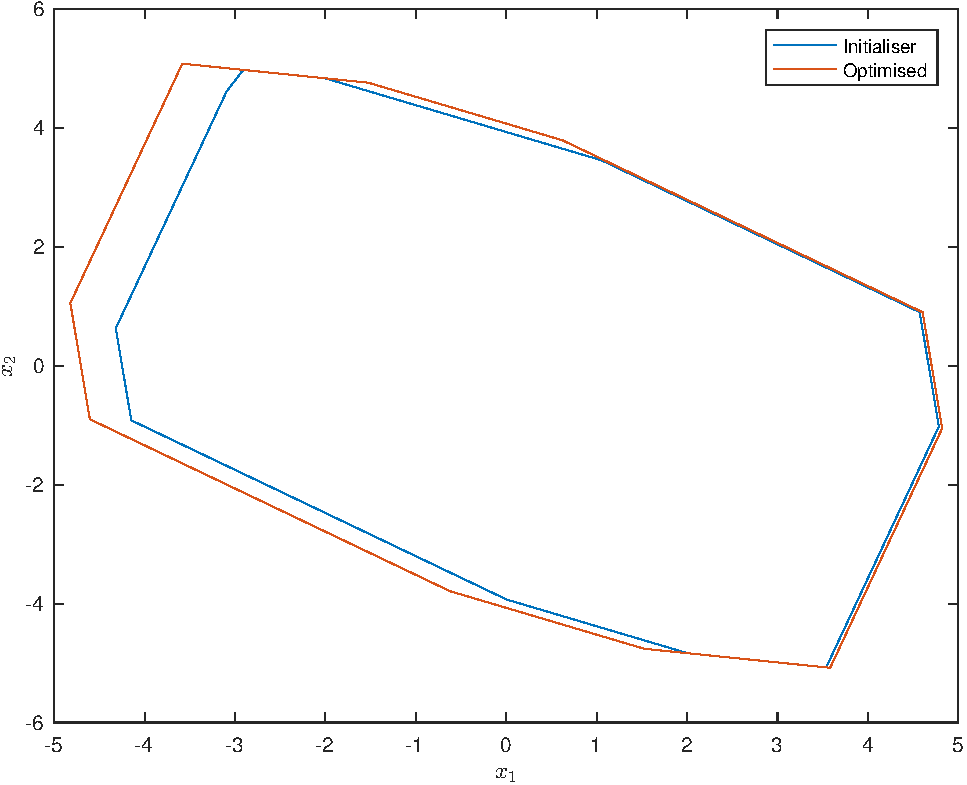
\includegraphics[width=.95\linewidth]{MRPIsetOptimised.pdf}
\caption{The guaranteed positive invariant set of the system~\eqref{eq:example:system:MRPI} in red, blue the robust positive invariant set for the disturbance set computed with the methods discussed in~\cite{Zhang2015}.}
\label{fig:MRPI:optimised}
\vspace{4mm}\end{figure}


For the same setup~\eqref{eq:example:system:MRPI} we approximate the guaranteed 3-step controllable set $\C_3(\T)$, where $\T=\{x:\norm{x}_\infty\leq 2\}$.
%
Again the result illustrated in figure~\ref{fig:n:step:controllable:set} can be reproduced using different initial values although the Hessian at the maximiser has a non-trivial nullspace.
%

\begin{figure}
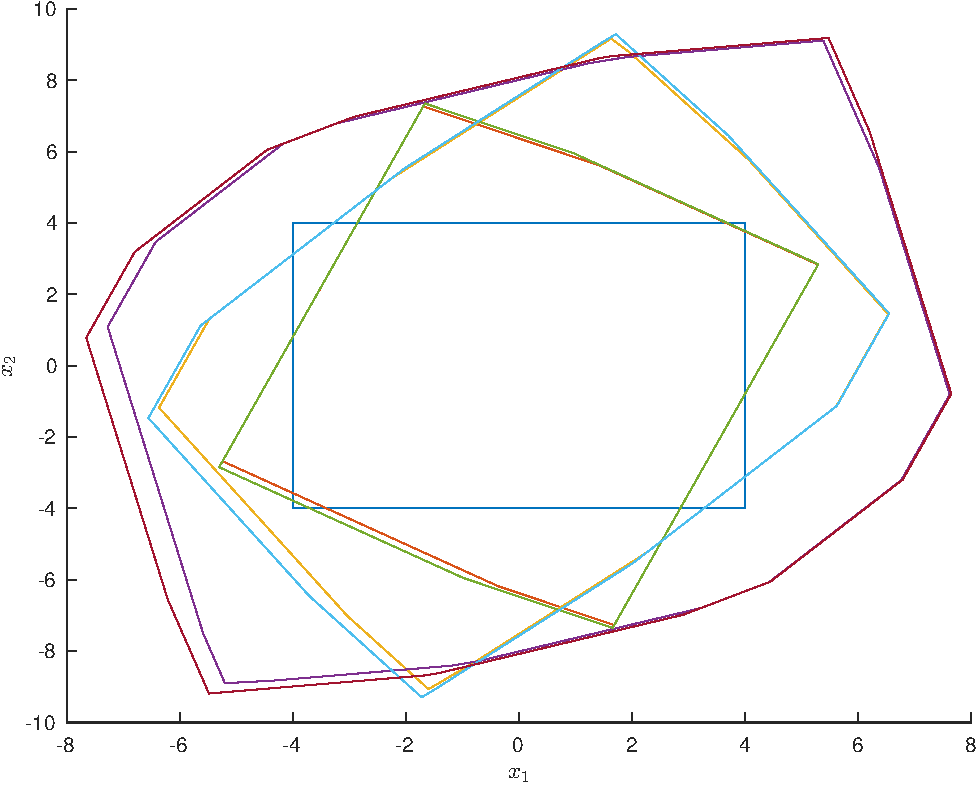
\includegraphics[width=.95\linewidth]{NStepSetOptimised.pdf}
\caption{Approximation of the guaranteed 3-step controllable set for a box $\T$ (in blue). The additional sets are remaining $C_1(\T),C_2(\T)$ and $C_3(\T)$ for the comparison set obtained with~\eqref{eq:comparison:set} and the optimised~$\V^\prime$ obtained with the proposed method.}
\label{fig:n:step:controllable:set}
\vspace{4mm}\end{figure}



\section{Conclusion}\label{sec:conclusion}
%
%
In this paper we presented a method in which the positive invariant set and the n-step controllable set of a stochastically constrained system are approximated respectively.
%
The method we present is based on a simple restriction of the set $\V^\prime\subseteq$ to be a parallelotope, which yields remarkable results in simulation and does not introduce non-convex constraints in the optimisation presented.
%
Although the presented scheme scales well to higher dimensions, the complexity of positive invariant sets and n-step controllable sets does not.
%
The underlying probability distribution was assumed to be uniform for ease of presentation, a similar method may be applied as long as the probability measure of a parallelotope can be analytically determined.
%
An additional improvement to the n-step controllable set $C_n(\T)$ could be obtained by introducing $\V_1^\prime,\dots,\V_{n-1}^\prime$, to allow different sets $\V_i^\prime$ at each stage introducing $(n-1)\times 2d$ additional decision variables.


%\bibliographystyle{alpha}
\bibliography{MyBibliography}
\end{document}